%
% $Id: ch02_relatedwork
%
%   *******************************************************************
%   * SEE THE MAIN FILE "AllegThesis.tex" FOR MORE INFORMATION.       *
%   *******************************************************************
\chapter{Related Work}\label{ch:relatedwork}

As expressed in the previous chapter, storage space on Internet accessible servers is at a premium when users have the ability to freely add content. In order to reduce the cost of operating image sharing websites it is necessary to develop and utilize technologies to reduce the space requirements. It is unsurprising that a large amount of research exists which targets the problem of locating similar images. Often, these comparison techniques were developed to be run on a local computer and not over the Internet, although the methods could be adapted to operate on a web based platform in many cases. By utilizing a combination of the research found in this chapter, it is possible to build a functional system capable of eliminating a large percentage of duplicate images on the server. When choosing a comparison method several characteristics were evaluated, namely efficiency, accuracy, and resource requirements.

\section{Primary Sources}
Although comparing existing images located in a database is not directly relevant to this research, the paper by Lee, Ke, and Isard \cite{Lee:2010} can be useful in method of approach. During their research they utilized a partition min-hash function for discovering near-duplicate images. Partition by hash functions are used to break down a large data set into a number of equal sized segments that can be identified by a generated hash. Instead of looking at the image as a whole as many other algorithms do, it looks at the image as several smaller pieces through the use of the partition hashing function. They claim that the algorithm is actually faster and more effective than standard functions which look at the entire image. Since the research is highly efficiency sensitive due to its web based structure, implementing a variant of this comparison method could prove beneficial. Even better, this research could be combined with research by Qu, Song, Yang, and Li where a new min-hash function was created called a spatial min-hash \cite{ZhangYinZhou}. Without too much detail, their algorithm is able to use traditional min-hash functions in combination with bag-of words technology to represent images in a more detailed and efficient manner \cite{Qu:2013:SMS:2499788.2499863}. In order to better understand this method, a brief overview of the bag-of-words model is needed. In its most basic form, this is an algorithm that looks at a set of data and groups the contents by category. In the discussion of images, these categories would be pixel values.

\begin{figure}[htbp]
\centering
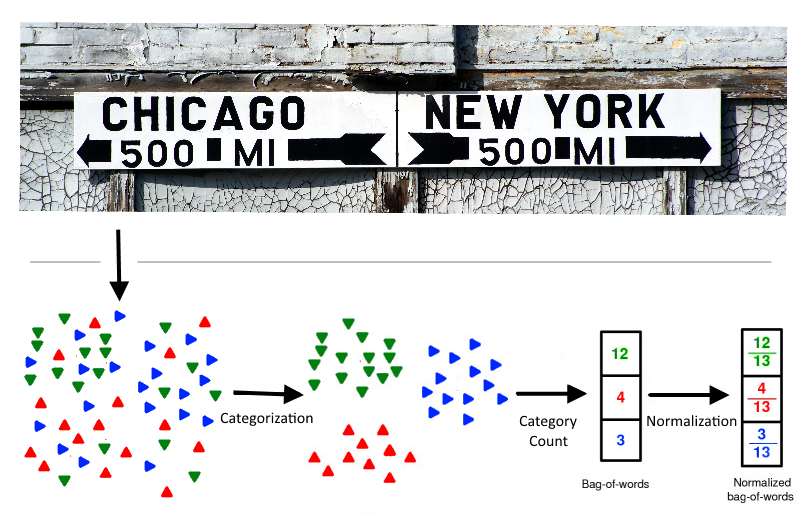
\includegraphics[width=5in]{bagofwords}
\caption{Visual breakdown of the bag-of-words algorithm.}
\label{bagofwords}
\end{figure}

As seen in Figure \ref{bagofwords}, this has been significantly simplified only showing one value of each red, green, and blue. An image will be broken down into a collection of all of its pixel colors as seen in the first step. Next, these values will be sorted into their appropriate groups. Again, this has been simplified to three categories for the purpose of visualization and in a real world scenario would potentially have thousands of color variations. Then, the algorithm looks at how many values are held in each grouping, giving a numeric representation of the values associated with each category. Finally, these frequency counts would be normalized with respect to the total number of values analyzed by the bag-of-words model \cite{ZhangYinZhou}. Note that the arbitrary value of 13 was selected for visualization purposes and has no significant meaning. By using this function combined with the previous paper's system, it would be possible to create an image de-duplication algorithm that has better performance and detection rates than one which implements only a traditional min-hash function.

Another article that is vital to creating an effective and efficient image matching algorithm is the 2010 paper by Srinivasan. This research was targeted at web-based image matching, which is directly related to this research. This research claims that traditional near-duplicate detection systems are not applicable for the de-duplication of large-scale web image collections \cite{Srinivasan:2008}, the research performed targeted an image matching system which was scalable, highly efficient, and effective.

In order to perform the effective image matching the authors required, they decided to implement a thumbnail matching based system. This algorithm would generate a 130-bit thumbnail representation of the image and was capable of finding near-duplicate images while operating in $O(1)$ time \cite{Srinivasan:2008}.

\begin{figure}[htbp]
\centering
\includegraphics[width=3.5in]{imagesamples}
\caption{Possible image manipulations.}
\label{imgsample}
\end{figure}

When using this thumbnail method, the authors were able to adjust automatically for differences in resolution, arbitrary amounts of cropping, caption, logo, and other manipulations, in addition to color and rotation variations, examples which can be seen in Figure \ref{imgsample}. Implementing a variant of this method was useful as each of these are highly probable manipulations in a real world scenario, and have been included in the final tests performed on the implemented system.

Due to the web based nature of the proposed research, another article, written by Foo, Zobel, Sinha, and Tahaghoghi in 2007 is highly related to the proposed research. This paper discusses the topic of web search based image matching \cite{Foo:2007}, mainly the finding and determination of types of copyright infringement as most near-duplicate images are derived from one source. The goal of their research was not to derive an algorithm capable of matching images, but to locate duplicate and near-duplicate images on the web using search engines, and determine the most common methods of image alteration leading to redundancy and possibly copyright infringement. Their research was invaluable to the proposed research as it allows targeting of the most common methods of image alteration when creating a matching algorithm. To locate their image set to work with, they used the most popular search queries of 2005 and collected the number of images, and determined the number of unique images based on the results returned. As a note, images with non-unique URLs were not included to prevent false duplicates from the same sites. In conclusion, the authors found that the most common alterations, ordered from one to 10, one being the most common, were as follows \cite{Foo:2007}:
\begin{enumerate}
\item
\textbf{Combination:} Images with more than one alteration.
\item
\textbf{Scale:} Images that differ in size.
\item
\textbf{Crop/Zoom:} Images that are cropped from the original.
\item
\textbf{Picture in Picture:} Images that contain another image.
\item
\textbf{Contrast:} Images that have adjusted contrast.
\item
\textbf{Border/Frame:} Images that have added borders or frames.
\item
\textbf{Grayscale:} Images that have been converted to grayscale.
\item
\textbf{Recoloring:} Images with colors that have been modified.
\item
\textbf{Mirror:} Images that have been mirrored to prevent copyright infringement detection.
\item
\textbf{Rotate:} Images that have been rotated.
\end{enumerate}

The research does not focus on every one of these common parameters that have been found, but will focus on a select group of these common alterations outlined in Section \ref{ch:reseval}.

Finally, the most relevant information found provides a starting codebase for the algorithm and research. An online coding tutorial provider, CatPa, outlined a method of using PHP libraries to generate real-time thumbnails and hashes of images and compare them to ones currently located on a server before uploading \cite{catpa:gdcode}. If the image is a duplicate it would be denied the privilege of being uploaded and the function would notify the user. This system is extremely limited as it provides the user with no way of adding an image to the server if it is not a duplicate and is only a false positive, and if it is unique, does not provide them with a method of accessing the already-present file.

The image comparison code developed by CatPa has been used as a base to generate a fully functional image sharing site with duplicate-reduction systems and allow for the testing of the effectiveness of such a system over traditional methods of sharing with duplicates allowed. The system created by the author \cite{catpa:gdcode} generates a $16\times 16$ thumbnail of each image on the server, and of the image being uploaded. From here, the algorithm generates and compares black and white and color histograms, the thumbnails, and determine if it is a duplicate based on the allowable difference threshold setting which was determined after running the initial tests outlined in Section \ref{ch:reseval} and analyzing the results \cite{catpa:gdcode}. The research utilizes this exact method, but also provides code improvements to utilize less memory by implementing the PHP Improved libraries and also checking images for immediate similarities in resolution and exact image matching with a full MD5 image hash. These methods require minimal calculation, just a simple comparison of strings compared to the generation of histograms and re-sizing of images. After the initial string comparison approach, the code was used to calculate an average deviation between two images and allows easy expansion of the system to provide a faster, more effective matching system.

\section{Additional Sources}
Throughout the entirety of this research project, one common theme that arises repeatedly is image re-sizing. Intuitively when an image is re-sized, the total number of pixels in the image is reduced or expanded. This means that the dimensions of the image have been manipulated. This process may seem fairly straightforward, but it is a huge area of research with many methods available to complete the same task. In the paper by Acharya and Tsai, they explain the meaning of image re-sizing as "...an image interpolation algorithm is used to convert an image from one resolution to another resolution without loosing the visual content in the picture." \cite{Acharya:2007}

The algorithms they mention come in two varieties, namely non-adaptive and adaptive. With non-adaptive algorithms, computations are performed to an entire image with no concern for the contents in it. Although the paper discusses several different algorithms, the detail of image manipulation would not have a significant impact on the research being completed. To better understand how image resizing works on the most basic level, two non-adaptive technologies will be briefly explored as seen in Figure \ref{interpolation}.

\begin{figure}[htbp]
\centering
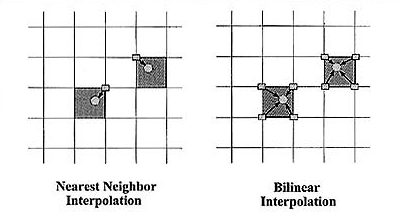
\includegraphics[width=3in]{interpolation}
\caption{Visual example of two basic non-adaptive algorithms.}
\label{interpolation}
\end{figure}

The first of the non-adaptive methods is called Nearest Neighbor Replacement. This is the most basic method available. When re-sizing an image using this method, the point being interpolated is replaced with only one of the surrounding pixels. This is very efficient and takes mearly no computational power to complete, but is is not recommended for images that must be of high quality. This is because upon completion of the process, the images tend to be pixelated in appearance \cite{Acharya:2007}.

The other method of image re-sizing is called Bilinear Interpolation. This method is also computationally efficient compared to other available methods, but it requires significantly more computational power than nearest neighbor replacement. As seen in Figure \ref{interpolation}, this method uses the four surrounding pixels to interpolate the pixel in question. The four surrounding pixels are weighted and used to determine the new pixel value. Again, this method is not particularly useful for high quality images as it tends to leave behind significant pixelation.

Finally, due to the fact that these methods are far too complex to briefly describe, the concept behind the category of algorithm will be analyzed. As seen above, non-adaptive technologies tend to leave poor quality images but have the strength of excellent performance. The trade off is great with adaptive algorithms where the computation power required is significantly more, though this category of algorithm typically provides a better quality manipulation. These algorithms operate in many ways sharing only the fact that they operate with respect to the content of the image. \cite{Wu:2007:NII:1777454.1777548} These algorithms exist to try and avoid image blurring, pixelation, loss of edge detail \cite{Centeno:2012:CAA:2245276.2245290}, artifacting, and more \cite{Acharya:2007}. The thumbnail producing technique employed in this research relies on a mixture of several non-adaptive image interpolation techniques to keep performance at its best.